% Options for packages loaded elsewhere
\PassOptionsToPackage{unicode}{hyperref}
\PassOptionsToPackage{hyphens}{url}
\PassOptionsToPackage{dvipsnames,svgnames,x11names}{xcolor}
%
\documentclass[
]{article}
\usepackage{amsmath,amssymb}
\usepackage{iftex}
\ifPDFTeX
  \usepackage[T1]{fontenc}
  \usepackage[utf8]{inputenc}
  \usepackage{textcomp} % provide euro and other symbols
\else % if luatex or xetex
  \usepackage{unicode-math} % this also loads fontspec
  \defaultfontfeatures{Scale=MatchLowercase}
  \defaultfontfeatures[\rmfamily]{Ligatures=TeX,Scale=1}
\fi
\usepackage{lmodern}
\ifPDFTeX\else
  % xetex/luatex font selection
\fi
% Use upquote if available, for straight quotes in verbatim environments
\IfFileExists{upquote.sty}{\usepackage{upquote}}{}
\IfFileExists{microtype.sty}{% use microtype if available
  \usepackage[]{microtype}
  \UseMicrotypeSet[protrusion]{basicmath} % disable protrusion for tt fonts
}{}
\makeatletter
\@ifundefined{KOMAClassName}{% if non-KOMA class
  \IfFileExists{parskip.sty}{%
    \usepackage{parskip}
  }{% else
    \setlength{\parindent}{0pt}
    \setlength{\parskip}{6pt plus 2pt minus 1pt}}
}{% if KOMA class
  \KOMAoptions{parskip=half}}
\makeatother
\usepackage{xcolor}
\usepackage[margin=1in]{geometry}
\usepackage{longtable,booktabs,array}
\usepackage{calc} % for calculating minipage widths
% Correct order of tables after \paragraph or \subparagraph
\usepackage{etoolbox}
\makeatletter
\patchcmd\longtable{\par}{\if@noskipsec\mbox{}\fi\par}{}{}
\makeatother
% Allow footnotes in longtable head/foot
\IfFileExists{footnotehyper.sty}{\usepackage{footnotehyper}}{\usepackage{footnote}}
\makesavenoteenv{longtable}
\usepackage{graphicx}
\makeatletter
\newsavebox\pandoc@box
\newcommand*\pandocbounded[1]{% scales image to fit in text height/width
  \sbox\pandoc@box{#1}%
  \Gscale@div\@tempa{\textheight}{\dimexpr\ht\pandoc@box+\dp\pandoc@box\relax}%
  \Gscale@div\@tempb{\linewidth}{\wd\pandoc@box}%
  \ifdim\@tempb\p@<\@tempa\p@\let\@tempa\@tempb\fi% select the smaller of both
  \ifdim\@tempa\p@<\p@\scalebox{\@tempa}{\usebox\pandoc@box}%
  \else\usebox{\pandoc@box}%
  \fi%
}
% Set default figure placement to htbp
\def\fps@figure{htbp}
\makeatother
\setlength{\emergencystretch}{3em} % prevent overfull lines
\providecommand{\tightlist}{%
  \setlength{\itemsep}{0pt}\setlength{\parskip}{0pt}}
\setcounter{secnumdepth}{5}
% definitions for citeproc citations
\NewDocumentCommand\citeproctext{}{}
\NewDocumentCommand\citeproc{mm}{%
  \begingroup\def\citeproctext{#2}\cite{#1}\endgroup}
\makeatletter
 % allow citations to break across lines
 \let\@cite@ofmt\@firstofone
 % avoid brackets around text for \cite:
 \def\@biblabel#1{}
 \def\@cite#1#2{{#1\if@tempswa , #2\fi}}
\makeatother
\newlength{\cslhangindent}
\setlength{\cslhangindent}{1.5em}
\newlength{\csllabelwidth}
\setlength{\csllabelwidth}{3em}
\newenvironment{CSLReferences}[2] % #1 hanging-indent, #2 entry-spacing
 {\begin{list}{}{%
  \setlength{\itemindent}{0pt}
  \setlength{\leftmargin}{0pt}
  \setlength{\parsep}{0pt}
  % turn on hanging indent if param 1 is 1
  \ifodd #1
   \setlength{\leftmargin}{\cslhangindent}
   \setlength{\itemindent}{-1\cslhangindent}
  \fi
  % set entry spacing
  \setlength{\itemsep}{#2\baselineskip}}}
 {\end{list}}
\usepackage{calc}
\newcommand{\CSLBlock}[1]{\hfill\break\parbox[t]{\linewidth}{\strut\ignorespaces#1\strut}}
\newcommand{\CSLLeftMargin}[1]{\parbox[t]{\csllabelwidth}{\strut#1\strut}}
\newcommand{\CSLRightInline}[1]{\parbox[t]{\linewidth - \csllabelwidth}{\strut#1\strut}}
\newcommand{\CSLIndent}[1]{\hspace{\cslhangindent}#1}
% \usepackage{booktabs}
\usepackage{bookmark}
\IfFileExists{xurl.sty}{\usepackage{xurl}}{} % add URL line breaks if available
\urlstyle{same}
\hypersetup{
  pdftitle={Causal Effect Estimation in Mendelian Randomisation Studies - Evaluating a Novel Bayesian Approach To Genetic Pleiotropy Versus Established Weighted Median Methodology},
  pdfauthor={B233241},
  colorlinks=true,
  linkcolor={Maroon},
  filecolor={Maroon},
  citecolor={Blue},
  urlcolor={blue},
  pdfcreator={LaTeX via pandoc}}

\title{Causal Effect Estimation in Mendelian Randomisation Studies - Evaluating a Novel Bayesian Approach To Genetic Pleiotropy Versus Established Weighted Median Methodology}
\author{B233241}
\date{September 2024 - June 2025}

\begin{document}
\maketitle

{
\hypersetup{linkcolor=}
\setcounter{tocdepth}{2}
\tableofcontents
}
\newpage

\subsection*{Acknowledgements}\label{acknowledgements}
\addcontentsline{toc}{subsection}{Acknowledgements}

I would like to acknowledge

\subsection*{Contributions}\label{contributions}
\addcontentsline{toc}{subsection}{Contributions}

Mine others

\subsection*{Statement of Originality}\label{statement-of-originality}
\addcontentsline{toc}{subsection}{Statement of Originality}

I confirm that all work is my own except where indicated, that all sources are clearly referenced\ldots.

\subsection*{Word Count}\label{word-count}
\addcontentsline{toc}{subsection}{Word Count}

Word count:
3166

\newpage

\section{Introduction and Background}\label{introduction-and-background}

\subsection{Introduction to Mendelian Randomisation (MR)}\label{introduction-to-mendelian-randomisation-mr}

Epidemiology is the study of determinants and distribution of disease across populations; a common epidemiological study aim is therefore to seek evidence as to whether a given exposure (e.g.~cigarette smoking) may cause a given outcome (e.g.~lung cancer)\textsuperscript{\citeproc{ref-coggon_chapter_2003}{1}}. Logistics limit experimental interventions across large groups, so insights into associations between exposures and outcomes are gleaned from observational data of people in the population of interest. Comparing health outcomes between individuals with different levels of a particular exposure may highlight potential links, e.g.~higher cancer incidence in those who smoke more is consistent with a causal role for cigarettes in carcinogenesis\textsuperscript{\citeproc{ref-coggon_chapter_2003}{1}}.

However, correlation does not prove causation. A key epidemiological challenge is accounting for so-called ``confounding'' factors; these are other variables, associated with both the exposure and the outcome of interest, which represent an alternative causal explanation for any exposure-outcome links observed\textsuperscript{\citeproc{ref-martens_instrumental_2006}{2}}. If smokers also drink more alcohol than non-smokers, then an observed link between smoking and increased cancer risk could plausibly be caused by increased alcohol exposure, either partially or entirely. Another potential issue with observational data is ``reverse causation'', where the presumed outcome is in fact a cause of the exposure; this might be the case if a cancer diagnosis drove individuals to drink and smoke more, and data were collected without respect to exposure timings.

\hyperref[acronyms_MR]{Mendelian randomisation (MR)} is a methodology intended to support causal inference from observational data. It applies the principles of instrumental variable (IV) analysis to genetic data, performing a type of natural experiment often likened to a randomised-controlled trial (RCT)\textsuperscript{\citeproc{ref-hernan_instruments_2006}{3}}.

In a properly conducted RCT, causality can be inferred due to a randomisation process being used as an ``instrument'' to allocate different levels of exposures to different experimental groups. If groups are randomly allocated, any confounding variables which might otherwise influence exposure-outcome relationships should be evenly distributed between groups, whether these confounders are known or not. As such, there should be no systematic differences between individuals from different groups in the exposure of interest - that is, there should be no bias\textsuperscript{\citeproc{ref-stel_instrumental_2013}{4}}. Statistical methods can quantify the probability that any observed outcome differences could have occurred by chance, and thereafter any outcome differences can be interpreted as caused by exposure differences. As allocation and receipt of exposures is known to precede outcome measurements, reverse causality is impossible.

In \hyperref[acronyms_MR]{MR}, naturally occurring genetic variants - ``genetic instruments'' -- are chosen based on their known association to an exposure of interest. Provided that assumptions of IV analysis are met, random assignment of genetic variants from parents to offspring during meiosis creates randomisation analagous to that performed for an RCT -- both measured and unmeasured confounders should be distributed evenly between the groups created, allowing valid causal inference after other sources of bias and random variation are accounted for\textsuperscript{\citeproc{ref-davies_reading_2018}{5}}.

\subsection{Causal Effect Estimation in MR}\label{causal-effect-estimation-in-mr}

At its simplest, the relationship between two continuous variables - an exposure \(X\) and outcome \(Y\) - can be represented as a linear model:

\begin{equation} 
Y = \alpha + \beta X + \epsilon
\end{equation}

where \(\alpha\) represents all non-\(X\) determinants of \(Y\), \(\beta\) is the causal effect of \(X\) on \(Y\) and \(\epsilon\) is an error term. The \(\beta\) term is a numerical measure of strength of causal exposure-outcome association, where:

\begin{itemize}
\tightlist
\item
  \(\beta = 0\) implies no causal link between exposure and outcome
\item
  \(\beta > 0\) implies \(X\) causes \(Y\)
\item
  \(\beta < 0\) implies \(X\) prevents \(Y\)
\end{itemize}

To estimate a causal effect using a genetic variant in an IV analysis, three key assumptions must be met\textsuperscript{\citeproc{ref-lousdal_introduction_2018}{6}}:

\begin{enumerate}
\def\labelenumi{\arabic{enumi}.}
\tightlist
\item
  Relevance -- the genetic variant must be associated with the exposure of interest
\item
  Independence -- the genetic variant is independent of confounders of the relationship between exposure and outcome
\item
  Exclusion restriction -- the genetic variant must not be associated with the outcome except via the exposure
\end{enumerate}

These assumptions are represented graphically in Figure \ref{fig:DAG-assumptions-plot}.

\begin{figure}
\centering
\pandocbounded{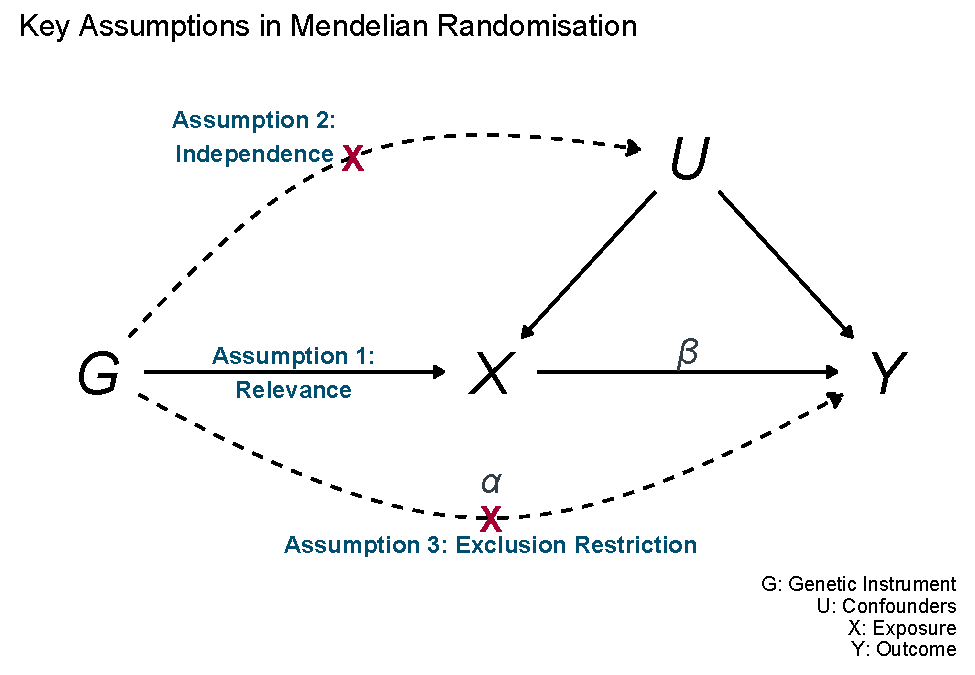
\includegraphics[keepaspectratio]{2_Intro_Background_files/figure-latex/DAG-assumptions-plot-1.pdf}}
\caption{\label{fig:DAG-assumptions-plot}Causal diagram illustrating the relationships between genetic instrument \emph{G}, exposure \emph{X}, outcome \emph{Y} and confounders of the exposure-outcome relationship \emph{U} in Mendelian randomisation studies. Blue text \& crosses represent key assumptions to ensure valid inference of causal effect of \emph{X} on \emph{Y} using \emph{G} as an instrumental variable. Red text represents violations of these assumptions that may lead to invalid inference through opening of alternate causal pathways. Greek characters represent the key parameters/association coefficients to be estimated. Adapted from Burgess et al 2016\textsuperscript{\citeproc{ref-burgess_sensitivity_2016}{7}}}
\end{figure}

Typically, MR studies estimate causal effect using a set of several genetic instruments; the causal effect estimate derived from the \(jth\) instrument is denoted \(\hat{\beta}_j\). Each estimate \(\hat{\beta}_j\) acknowledges there will be specific effects on the observed values of exposure and outcome given the presence of that specific genetic variable \(G_j\) under study, i.e.~\(\hat{\beta}_j\) is based on the observed exposure \({X|G_j}\) and outcome \({Y|G_j}\). These observed values of exposure and outcome can be described by their own linear models:

\begin{equation} 
X|G_j = \gamma_0 + \gamma_j G_j + \epsilon_{X_j}
\end{equation}

\begin{equation} 
Y|G_j = \Gamma_0 + \Gamma_j G_j + \epsilon_{Y_j}
\end{equation}

where, for exposure and outcome respectively:

\begin{itemize}
\tightlist
\item
  \(\gamma_0\) and \(\Gamma_0\) reflect base values without influence of the genetic variant
\item
  \(\gamma_j\) and \(\Gamma_j\) are coefficients of association with the genetic variant, representing the extent to which an effect allele of \(G_j\) will perturb the value of \(X\) or \(Y\) versus the non-effect allele
\item
  \(\epsilon_{X_j}\) and \(\epsilon_{Y_j}\) are error terms, containing contributions from confounders of the exposure-outcome relationship (\(U\) in the causal diagram), and all genetic variants except \(G_j\).
\end{itemize}

It can be shown that a simple causal effect estimate for the exposure on the outcome can be obtained from a single genetic instrument by the Wald method, dividing the coefficient of gene-outcome association by the coefficient of gene-exposure association, i.e.:

\begin{equation} 
\hat{\beta}_j = \frac {\hat{\Gamma}_j} {\hat{\gamma}_j}
\end{equation}

Each instrument may be valid or invalid, depending on it meeting the above assumptions. The overall causal effect estimate \(\hat{\beta}\) from any given MR method will typically seek to pool effect estimates from several instruments so as to minimise effects of any invalid instruments included, e.g.~by removing/down-weighting contributions of genetic instruments which violate one or more assumptions. This is equivalent to plotting all estimated coefficients of gene-outcome association (\(\bar{\Gamma}\)) versus all estimated coefficients of gene-exposure association (\(\bar{\gamma}\)) for the set of instruments, then using the gradient of a regression line through the points as the causal effect estimate \(\hat{\beta}\); picking an MR methodology is analogous to choosing the method to draw the line of best fit (Figure \ref{fig:Gamma-gamma-plot}). For binary outcomes, the causal effect estimate can be converted to an odds ratio (OR) through exponentiation, i.e.:

\begin{equation} 
OR = e^{\hat{\beta}}
\end{equation}

\begin{figure}
\centering
\pandocbounded{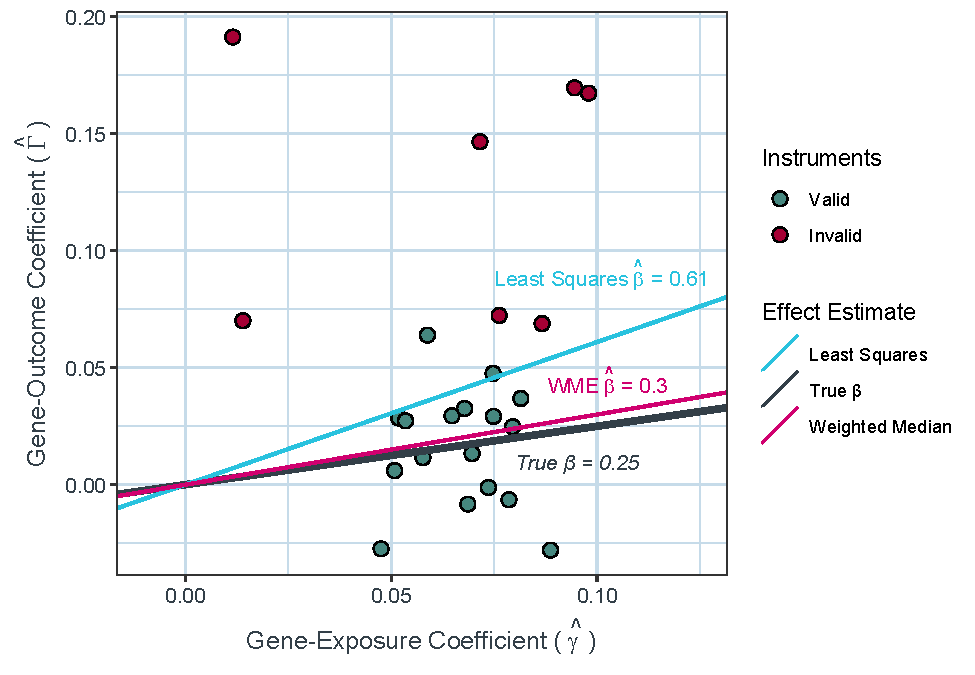
\includegraphics[keepaspectratio]{2_Intro_Background_files/figure-latex/Gamma-gamma-plot-1.pdf}}
\caption{\label{fig:Gamma-gamma-plot}Simulated MR Study on 10,000 individuals using 25 genetic instruments, of which 30\% are invalid (red points) and introduce directional pleiotropic effects. The true value of the exposure-outcome causal effect is 0.25 (grey line, causal effect represented by gradient). Regression using an unajusted least-squares linear model (light blue line) results in a biased estimate in the positive direction due to the influence of the invalid instruments. Using the Weighted Median Estimator method (pink line) attenuates the effects of the invalid instruments, resulting in an estimate closer to the true value. Adapted from Bowden et al 2016\textsuperscript{\citeproc{ref-bowden_consistent_2016}{8}}}
\end{figure}

\subsection{Violations to Assumptions}\label{violations-to-assumptions}

In practice, only the relevance assumption can be directly tested and proven. Typically, genetic variants for MR studies are selected as instruments based on Genome Wide Association Studies (GWAS), which quantify associations between genetic Single Nucleotide Polymorphisms (SNPs) and various phenotypes. Association between genetic variants and a phenotypes representing exposures of interest can be partly assured by selection using an appropriate genome-wide significance level (e.g.~\(p < 10 ^{-8}\)). Statistical testing can also quantify the gene-exposure relationship; commonly used measures include the \(r^2\) statistic, representing the proportion of variance in the exposure explained by the genotype, and the related \(F\)-statistic, which additionally accounts for the the sample size under investigation\textsuperscript{\citeproc{ref-richmond_mendelian_2022}{9}}. An \(F\)-statistic of \(\ge\) 10 is generally considered to represent a strong enough gene-exposure association to consider a genetic instrument for use\textsuperscript{\citeproc{ref-martens_instrumental_2006}{2}}.

The assumptions of independence and exclusion restriction depend on all possible confounders of the exposure-outcome association, both measured and unmeasured; as such, these can never be proven absolutely. Various methods have been proposed to quantify and account for violations of these two additional assumptions, including the weighted median estimator, described below\textsuperscript{\citeproc{ref-bowden_consistent_2016}{8}}.

The main methods to avoid violations of the independence assumption relate to appropriate selection of populations studied to avoid confounding due to ancestry or population stratification. For example, in two-sample MR studies, where gene-exposure and gene-outcome coefficients are estimated from two separate GWAS studies, it is recommended to select GWAS studies performed in similar population groups (e.g.~both in Western Europeans). This practice helps avoid spurious exposure-outcome associations being generated by confounding due to underlying differences in allele frequency, baseline disease risks etc between different populations\textsuperscript{\citeproc{ref-richmond_mendelian_2022}{9}}.

Exclusion restriction is a particularly universal issue in MR, due to so-called (horizontal) genetic pleiotropy, where a single genetic variant may have multiple ``pleiotropic'' effects -- i.e.~it may influence several traits simultaneously. Such pleiotropic effects may be unknown and open unmeasured causal pathways between a genetic instrument and the outcome, thus potentially biasing MR estimates of the association between exposure and outcome. As pleiotropy influences outcome separate to the path involving the exposure of interest, the term ``direct effects'' is also used\textsuperscript{\citeproc{ref-hemani_evaluating_2018}{10}}. Where pleiotropic effects are in both positive and negative directions with a mean of zero - ``balanced pleiotropy'' - then they only add noise to causal effect estimation\textsuperscript{\citeproc{ref-morrison_mendelian_2020}{11}}. By contrast, ``directional pleiotropy'', where the mean of pleiotropic effects is non-zero, may introduce bias\textsuperscript{\citeproc{ref-bowden_consistent_2016}{8}}.

If such an additional causal pathway acts between gene \(G\) and outcome \(Y\) via a confounding factor \(U\), then the magnitude of direct/overall effects of \(G\) on \(Y\) will correlate with the effects of \(G\) on \(X\) (i.e.~\(\Gamma \propto \gamma\)), and ``correlated pleiotropy'' is present. If an additional causal pathway acts directly between gene \(G\) and outcome \(Y\) independent of both exposure \(X\) and confounders \(U\), this results in ``uncorrelated pleiotropy'' (Figure \ref{fig:DAG-assumptions-plot}). Both correlated and uncorrelated pleiotropy can introduce bias which distorts the estimate of the true causal effect. In general, correlated pleiotropy is more challenging to account for; several MR methods explicitly require an additional assumption of Instrument Strength Independent of Direct Effects (the InSIDE assumption), i.e no correlated pleiotropy to be present\textsuperscript{\citeproc{ref-grant_bayesian_2024}{12}}.

\subsection{Weighted Median Estimator (WME)}\label{weighted-median-estimator-wme}

A common approach to produce exposure-outcome causal effect estimates robust to violations of the exclusion restriction assumption is the Weighted Median Estimator (WME) method, proposed by Bowden et al\textsuperscript{\citeproc{ref-bowden_consistent_2016}{8}}.

In WME analysis, several genetic instruments are used to estimate the exposure-outcome causal effect \(\hat{\beta}\). Each instrument is known to be associated with the exposure of interest, but an unknown proportion of these instruments may be invalid due to pleiotropic genetic effects. Any instrument linked to an outcome via multiple pleiotropic causal pathways will exhibit a less consistent gene-outcome association than a relationship mediated by a single pathway; this results in larger variance in causal estimates derived from invalid/pleiotropic genetic instruments versus estimates from valid instruments.

WME therefore assigns a weight to each genetic instrument's estimate of the causal effect according to the inverse of the variance of the estimate; these weighted effect estimates are used to construct a cumulative distribution function for probability of true causal effect size across the range of estimated values. The 50th percentile of this distribution can then be taken as a ``weighted median estimate'' of the true causal effect, theoretically producing consistent causal estimates even if up to 50\% of the included information comes from invalid instruments\textsuperscript{\citeproc{ref-bowden_consistent_2016}{8}}. An example of WME attenuating the effects of invalid instruments is shown in Figure \ref{fig:Gamma-gamma-plot}.

\subsection{Issues With WME}\label{issues-with-wme}

WME calculation methods are available via several prolific MR tools: the R packages ``MendelianRandomization''\textsuperscript{\citeproc{ref-yavorska_mendelianrandomization_2017}{13}} and ``TwoSampleMR'', and the MR-Base web platform\textsuperscript{\citeproc{ref-hemani_mr-base_2018}{14}}. However, these implement the original authors' suggested process of generating 95\% confidence intervals for WME, which deviates from accepted resampling methodology:

\begin{quote}
``We found the bootstrap confidence interval\ldots too conservative. However, the bootstrap standard error\ldots{} gave more reasonable coverage using a normal approximation (estimate ±1.96 x standard error) to form a 95\% confidence interval''\textsuperscript{\citeproc{ref-bowden_consistent_2016}{8}}
\end{quote}

This modification, explicitly aiming to boost estimate precision artificially, would be expected to lead to a high Type 1 error rate, which has been a growing concern in the field of late\textsuperscript{\citeproc{ref-stender_reclaiming_2024}{15}}.

\subsection{MR-Hevo}\label{mr-hevo}

MR-Hevo\textsuperscript{\citeproc{ref-mckeigue_inference_2024}{16}} is an R package which uses more typical Bayesian methodology to estimate MR causal effects and corresponding 95\% confidence intervals. It uses the probabilistic programming language, Stan, to directly sample the posterior probability distribution of pleiotropic effects on the outcome, rather than assuming that this distribution can be simulated as Gaussian, as current WME implementations do. MR-Hevo also handles multiple instruments per genetic locus via scalar construction, and specifies a prior probability distribution which reflects prior knowledge that most individual genetic instruments will have only small effects on complex traits\textsuperscript{\citeproc{ref-park_estimation_2010}{17},\citeproc{ref-piironen_sparsity_2017}{18}}, further aiding biologically plausible inference regarding distribution of pleiotropic effects.

The main aim of this study will be to demonstrate if the WME approach gives over-confident causal estimates in the presence of pleiotropy, and whether this issue is more correctly handled by the MR-Hevo Bayesian approach.

\newpage

\section{References}\label{references}

\phantomsection\label{refs}
\begin{CSLReferences}{0}{1}
\bibitem[\citeproctext]{ref-coggon_chapter_2003}
\CSLLeftMargin{1. }%
\CSLRightInline{Coggon D, Rose G, Barker D. Chapter 1. {What} is epidemiology? {\textbar} {The} {BMJ}. In: The {BMJ} {\textbar} {The} {BMJ}: Leading general medical journal {Research} {Education} {Comment} {[}Internet{]}. 2003 {[}cited 2025 Apr 29{]}. Available from: \url{https://www.bmj.com/about-bmj/resources-readers/publications/epidemiology-uninitiated/1-what-epidemiology}}

\bibitem[\citeproctext]{ref-martens_instrumental_2006}
\CSLLeftMargin{2. }%
\CSLRightInline{Martens EP, Pestman WR, Boer A de, Belitser SV, Klungel OH. Instrumental {Variables}: {Application} and {Limitations}. Epidemiology {[}Internet{]}. 2006 May {[}cited 2025 Apr 29{]};17(3):260. Available from: \url{https://journals.lww.com/epidem/fulltext/2006/05000/instrumental_variables__application_and.10.aspx}}

\bibitem[\citeproctext]{ref-hernan_instruments_2006}
\CSLLeftMargin{3. }%
\CSLRightInline{Hernán MA, Robins JM. Instruments for {Causal} {Inference}: {An} {Epidemiologist}'s {Dream}? Epidemiology {[}Internet{]}. 2006 Jul {[}cited 2025 Apr 29{]};17(4):360. Available from: \url{https://journals.lww.com/epidem/fulltext/2006/07000/instruments_for_causal_inference__an.4.aspx\#JCL1-2}}

\bibitem[\citeproctext]{ref-stel_instrumental_2013}
\CSLLeftMargin{4. }%
\CSLRightInline{Stel VS, Dekker FW, Zoccali C, Jager KJ. Instrumental variable analysis. Nephrology Dialysis Transplantation {[}Internet{]}. 2013 Jul {[}cited 2025 Apr 29{]};28(7):1694--9. Available from: \url{https://doi.org/10.1093/ndt/gfs310}}

\bibitem[\citeproctext]{ref-davies_reading_2018}
\CSLLeftMargin{5. }%
\CSLRightInline{Davies NM, Holmes MV, Smith GD. Reading {Mendelian} randomisation studies: A guide, glossary, and checklist for clinicians. BMJ {[}Internet{]}. 2018 Jul {[}cited 2025 Jan 7{]};362:k601. Available from: \url{https://www.bmj.com/content/362/bmj.k601}}

\bibitem[\citeproctext]{ref-lousdal_introduction_2018}
\CSLLeftMargin{6. }%
\CSLRightInline{Lousdal ML. An introduction to instrumental variable assumptions, validation and estimation. Emerging Themes in Epidemiology {[}Internet{]}. 2018 Jan {[}cited 2025 Apr 29{]};15:1. Available from: \url{https://www.ncbi.nlm.nih.gov/pmc/articles/PMC5776781/}}

\bibitem[\citeproctext]{ref-burgess_sensitivity_2016}
\CSLLeftMargin{7. }%
\CSLRightInline{Burgess S, Bowden J, Fall T, Ingelsson E, Thompson SG. Sensitivity {Analyses} for {Robust} {Causal} {Inference} from {Mendelian} {Randomization} {Analyses} with {Multiple} {Genetic} {Variants}. Epidemiology (Cambridge, Mass) {[}Internet{]}. 2016 Nov {[}cited 2024 Oct 22{]};28(1):30. Available from: \url{https://pmc.ncbi.nlm.nih.gov/articles/PMC5133381/}}

\bibitem[\citeproctext]{ref-bowden_consistent_2016}
\CSLLeftMargin{8. }%
\CSLRightInline{Bowden J, Smith GD, Haycock PC, Burgess S. Consistent {Estimation} in {Mendelian} {Randomization} with {Some} {Invalid} {Instruments} {Using} a {Weighted} {Median} {Estimator}. Genetic Epidemiology {[}Internet{]}. 2016 Apr {[}cited 2024 Oct 22{]};40(4):304. Available from: \url{https://pmc.ncbi.nlm.nih.gov/articles/PMC4849733/}}

\bibitem[\citeproctext]{ref-richmond_mendelian_2022}
\CSLLeftMargin{9. }%
\CSLRightInline{Richmond RC, Smith GD. Mendelian {Randomization}: {Concepts} and {Scope}. Cold Spring Harbor Perspectives in Medicine {[}Internet{]}. 2022 Jan {[}cited 2024 Oct 22{]};12(1):a040501. Available from: \url{https://pmc.ncbi.nlm.nih.gov/articles/PMC8725623/}}

\bibitem[\citeproctext]{ref-hemani_evaluating_2018}
\CSLLeftMargin{10. }%
\CSLRightInline{Hemani G, Bowden J, Smith GD. Evaluating the potential role of pleiotropy in {Mendelian} randomization studies. Human Molecular Genetics {[}Internet{]}. 2018 May {[}cited 2024 Oct 23{]};27(R2):R195. Available from: \url{https://pmc.ncbi.nlm.nih.gov/articles/PMC6061876/}}

\bibitem[\citeproctext]{ref-morrison_mendelian_2020}
\CSLLeftMargin{11. }%
\CSLRightInline{Morrison J, Knoblauch N, Marcus JH, Stephens M, He X. Mendelian randomization accounting for correlated and uncorrelated pleiotropic effects using genome-wide summary statistics. Nature Genetics {[}Internet{]}. 2020 Jul {[}cited 2025 May 22{]};52(7):740--7. Available from: \url{https://www.nature.com/articles/s41588-020-0631-4}}

\bibitem[\citeproctext]{ref-grant_bayesian_2024}
\CSLLeftMargin{12. }%
\CSLRightInline{Grant AJ, Burgess S. A {Bayesian} approach to {Mendelian} randomization using summary statistics in the univariable and multivariable settings with correlated pleiotropy. The American Journal of Human Genetics {[}Internet{]}. 2024 Jan {[}cited 2025 May 20{]};111(1):165--80. Available from: \url{https://www.cell.com/ajhg/abstract/S0002-9297(23)00433-0}}

\bibitem[\citeproctext]{ref-yavorska_mendelianrandomization_2017}
\CSLLeftMargin{13. }%
\CSLRightInline{Yavorska OO, Burgess S. {MendelianRandomization}: An {R} package for performing {Mendelian} randomization analyses using summarized data. International Journal of Epidemiology {[}Internet{]}. 2017 Dec {[}cited 2024 Oct 23{]};46(6):1734--9. Available from: \url{https://doi.org/10.1093/ije/dyx034}}

\bibitem[\citeproctext]{ref-hemani_mr-base_2018}
\CSLLeftMargin{14. }%
\CSLRightInline{Hemani G, Zheng J, Elsworth B, Wade KH, Haberland V, Baird D, et al. The {MR}-{Base} platform supports systematic causal inference across the human phenome. Loos R, editor. eLife {[}Internet{]}. 2018 May {[}cited 2025 Jan 7{]};7:e34408. Available from: \url{https://doi.org/10.7554/eLife.34408}}

\bibitem[\citeproctext]{ref-stender_reclaiming_2024}
\CSLLeftMargin{15. }%
\CSLRightInline{Stender S, Gellert-Kristensen H, Smith GD. Reclaiming mendelian randomization from the deluge of papers and misleading findings. Lipids in Health and Disease {[}Internet{]}. 2024 Sep {[}cited 2025 Jan 7{]};23(1):286. Available from: \url{https://doi.org/10.1186/s12944-024-02284-w}}

\bibitem[\citeproctext]{ref-mckeigue_inference_2024}
\CSLLeftMargin{16. }%
\CSLRightInline{McKeigue PM, Iakovliev A, Spiliopoulou A, Erabadda B, Colhoun HM. Inference of causal and pleiotropic effects with multiple weak genetic instruments: Application to effect of adiponectin on type 2 diabetes {[}Internet{]}. medRxiv; 2024 {[}cited 2024 Oct 23{]}. Available from: \url{https://www.medrxiv.org/content/10.1101/2023.12.15.23300008v2}}

\bibitem[\citeproctext]{ref-park_estimation_2010}
\CSLLeftMargin{17. }%
\CSLRightInline{Park JH, Wacholder S, Gail MH, Peters U, Jacobs KB, Chanock SJ, et al. Estimation of effect size distribution from genome-wide association studies and implications for future discoveries. Nature genetics {[}Internet{]}. 2010 Jun {[}cited 2024 Oct 23{]};42(7):570. Available from: \url{https://pmc.ncbi.nlm.nih.gov/articles/PMC4615599/}}

\bibitem[\citeproctext]{ref-piironen_sparsity_2017}
\CSLLeftMargin{18. }%
\CSLRightInline{Piironen J, Vehtari A. Sparsity information and regularization in the horseshoe and other shrinkage priors. Electronic Journal of Statistics {[}Internet{]}. 2017 Jan {[}cited 2025 Jan 7{]};11(2):5018--51. Available from: \url{https://projecteuclid.org/journals/electronic-journal-of-statistics/volume-11/issue-2/Sparsity-information-and-regularization-in-the-horseshoe-and-other-shrinkage/10.1214/17-EJS1337SI.full}}

\end{CSLReferences}

\appendix


\newpage

\section{Appendix A: List of Abbreviations}\label{appendix-a-list-of-abbreviations}

\begin{description}
\tightlist
\item[\phantomsection\label{acronyms_MR}{MR}]
Mendelian randomisation
\end{description}

\newpage

\section{Appendix B: Simulation Code}\label{appendix-b-simulation-code}

\subsubsection{Generating Data and Models}\label{generating-data-and-models}

The data generating model used was from Appendix 3 of Bowden et al (ref); the relevant section describing their model is reproduced below:

\emph{``\ldots{}}

\begin{equation}
 U_i = \sum^J_{j=1} \phi_jG_{ij} + \epsilon_i^U
 \end{equation}

\begin{equation}
 X_i = \sum^J_{j=1} \gamma_jG_{ij} + U_i + \epsilon_i^X
 \end{equation}

\begin{equation}
 Y_i = \sum^J_{j=1} \alpha_jG_{ij} + \beta X_i + U_i + \epsilon_i^Y
 \end{equation}

\emph{for participants indexed by \(i = 1, . . . , N\), and genetic instruments indexed by \(j = 1, . . . , J\).}

\emph{The error terms \(\epsilon_i^U , \epsilon_i^X\) and \(\epsilon_i^Y\) were each drawn independently from standard normal distributions. The genetic effects on the xposure γj are drawn from a uniform distribution between 0.03 and 0.1. Pleiotropic effects \(\alpha_j\) and \(\phi_j\) were set to zero if the genetic instrument was a alid instrumental variable. Otherwise (with probability 0.1, 0.2, or 0.3):}

\emph{1. In Scenario 1 (balanced pleiotropy, InSIDE satisfied), the \(\alpha_j\) parameter was drawn from a uniform distribution between −0.2 and 0.2.}

\emph{2. In Scenario 2 (directional pleiotropy, InSIDE satisfied), the \(\alpha_j\) parameter was drawn from a uniform distribution between 0 and 0.2.}

\emph{3. In Scenario 3 (directional pleiotropy, InSIDE not satisfied), the \(\phi_j\) parameter was drawn from a uniform distribution between −0.2 and 0.2.}

\emph{The causal effect of the exposure on the outcome was either \(\beta X = 0\) (null causal effect) or \(\beta X = 0.1\) (positive causal effect). A total of 10 000 simulated datasets were generated for sample sizes of N = 10 000 and 20 {[}sic{]} participants. Only the summary data, that is genetic associations with the exposure and with the outcome and their standard errors as estimated by univariate regression on the genetic instruments in turn, were used by the analysis methods. In the two-sample setting, data were generated on 2N participants, and genetic associations with the exposure were estimated in the first N participants, and genetic associations with the outcome in the second N participants.''}\textsuperscript{\citeproc{ref-bowden_consistent_2016}{8}}

To reproduce this model, code was written in R to generate the relevant participant level data. First, a function (\texttt{simulate\_MR\_data}) was written which included arameters specified by Bowden et al, and also to allow testing of data simulation:

This initial simulation function generated data in the following format:

A function (\texttt{extract\_models}) was then written to create linear models from each dataset generated as per Bowden et al:

These models generated estimates of the coefficient of gene:exposure association (\texttt{coeff\_G\_X}), coefficient of gene:outcome association (\texttt{coeff\_G\_Y}), and the elevant standard errors of these estimates. The values of parameters inputted were also returned to aid in further testing of data/model generation, i.e.~actual ene:exposure associations (\texttt{gamma}), pleiotropic effects of invalid instruments (\texttt{alpha}), additional pleiotropic effects when InSIDE assumption not satified \texttt{phi}), causal effect of exposure on outcome (\texttt{beta}) and the proportion of invalid genetic instruments with pleiotropic effects on the outcome (\texttt{prop\_invalid}).

\subsubsection{Testing Generation of Data and Models}\label{testing-generation-of-data-and-models}

A series of test plots were used to verify that data were simulated as intended under the various conditions specified by input parameters. Test plots were not reated for the parameters \texttt{n\_participants}, \texttt{n\_instruments} or \texttt{n\_datasets}, as the functioning of these parameters could be readily inferred from the structure of he datasets outputted, as above.

The \texttt{prop\_invalid} parameter specifies the proportion of invalid genetic instruments simulated, i.e.~the proportion of genetic instruments affecting the outcome via irect/pleiotropic effects, and thus not solely via the exposure of interest. If simulated correctly, increasing the value of \texttt{prop\_invalid} should increase the umber of instruments with pleiotropic effects, i.e.~instruments with \texttt{alpha} =/= 0. With random error terms set to 0 and no causal effect present (i.e.~\texttt{rand\_error\ =\ ALSE} and \texttt{causal\_effect\ =\ FALSE}), the estimated gene:outcome coefficient estimated using any given instrument will equal the pleiotropic effects of that instrument i.e.~\texttt{coeff\_G\_Y\ =\ alpha}), and therefore will only be non-zero for invalid instruments with non-zero pleiotropic effects on the outcome . Plotting \texttt{coeff\_G\_Y} gainst \texttt{alpha} for simulated data with no causal effect or random error should therefore yield a graph where

\begin{itemize}
\tightlist
\item
  For valid instruments: gene:outcome coefficient = alpha = 0
\item
  For invalid instruments: gene:outcome coefficient = alpha =/= 0, with values spread uniformly between \texttt{alpha\_min} and \texttt{alpha\_max}
\end{itemize}

Similarly, with random error terms set to 0 and no causal effect present, gene:exposure coefficients estimated for each instrument should exactly match the actual alues simulated, i.e.~\texttt{coeff\_G\_X\ =\ gamma} for all instruments:

For the next phase of testing, a function (\texttt{plot\_GY\_GX}) was written to plot the coefficients for gene:exposure versus gene:outcome as estimated using the reviously created linear models:

\newpage

\section{Appendix C: Citation Search Strategy}\label{appendix-c-citation-search-strategy}

\end{document}
